\documentclass{ifacconf}
\usepackage{standalone}
\usepackage{times}
\usepackage{float}
\usepackage{amsmath}
\usepackage{graphicx}      % include this line if your document contains figures
\usepackage{natbib}        % required for bibliography
%===========================================
%\documentclass[letterpaper, 11pt, onecolumn]{TemplateFiles/ieeeconf}
%\IEEEoverridecommandlockouts \overrideIEEEmargins 
%\pagestyle{plain}

%\usepackage[ruled,vlined,linesnumbered,boxruled]{algorithm2e}
%\usepackage{mathrsfs}
%\usepackage{graphicx}
%\usepackage{amsfonts}
%\usepackage{amsmath}
%\usepackage{amssymb}
%\usepackage{array}
%\usepackage{flafter}
%\usepackage{tabu}
%\usepackage{cite}
%\usepackage{subfigure}
%\usepackage{verbatim}
%\usepackage{bbm}
%\usepackage[usenames]{color}
%\usepackage[svgnames]{xcolor}

%\usepackage{balance}

%\usepackage{nicefrac}
%\usepackage{psfrag}
%\usepackage{umoline}
%\usepackage{hyperref}
%\usepackage{appendix} %[2009/09/02 v1.2b extra appendix facilities]
%\let\proof\relax
%\let\endproof\relax
%\usepackage{amsthm}	% This is needed for \newtheorem and proof environment.
% \usepackage{natbib} % for citing the papers with auther-year format in parantheses.
%\usepackage[numbers, sort]{natbib}

%\usepackage{etoolbox}

%\providecommand{\citet}[1]{\citeauthor{#1}\,[\citeyear{#1}]}
%\providecommand{\citep}[1]{\cite{#1}}

%\newtheorem{thm}{Theorem}
%\newtheorem{Def}{Definition}
%\newtheorem{Problem}{Problem}
%\newtheorem{Lem}{Lemma}
%\newtheorem{Cor}{Corollary}
%\newtheorem{assumption}{Assumption}
%\newtheorem{proposition}{Proposition}
%\newtheorem{definition}{Definition}
%\newtheorem{property}{Property}
%\newtheorem{Remark}{Remark}
%\newtheorem{exmp}{Example}[section]
%\newenvironment{proof}[1][Proof]{\begin{trivlist}
%\item[\hskip \labelsep {\bfseries #1}]}{\end{trivlist}}

%\newcommand{\TypeOfDoc}{IJRR} % This either can be TR or Conf or IJRR
%\newcommand{\FinalFlag}{No} % This either can be No or Accepted
%\newtoggle{finalpaper}
%\toggletrue{finalpaper}
%\togglefalse{finalpaper}

\graphicspath{{./figs/}}

%\allowdisplaybreaks[1]

%\newcommand{\kXX}[1]{\color{blue} XX #1 XX \color{black}}
%newcommand{\AXX}[1]{\color{purple} XX #1 XX \color{black}}
\newcommand{\aXX}[1]{\color{orange} #1  \color{black}}
\newcommand{\axx}[1]{\aXX{#1}}


\newcommand{\pr}[1]{\textbf{#1:} }

\newcommand{\codeline}[1]{\par{\ttfamily #1 \par}}  % This line is added because sth like this \newcommand{\initeali}{\verb|InitializeEdge|} does not work. For further details please check out this link % http://tex.stackexchange.com/questions/86071/newcommand-for-verbatim
% please do not delete above comments as it can be really confsing


%%%%%%%%%%%%%%%% symbols
\newcommand{\tv}{\varpi} % tube volume (edge tube volume)
\newcommand{\td}{\Gamma} % tube distance (edge tube distance)

%%%%%%%%%%%%%%%%%%%%%%%%%%%%%%%%%%%%%%%%%%%%%%%%%% To reduce pages
%\textfloatsep = 0pt
%\renewcommand{\baselinestretch}{0.96}
%%%%%%%%%%%%%%%%% Make bibs smaller
%\renewcommand{\IEEEbibitemsep}{0pt plus 2pt}
%\makeatletter
%\IEEEtriggercmd{\reset@font\normalfont\footnotesize}
%\makeatother
%\IEEEtriggeratref{1}

%%%%%%%%%%%%%%%%% margins
%\usepackage{geometry}
% \newcommand{\papermargin}{0.97in} % IEEE asks for 0.75 on all pages, but the first page
% %\newgeometry{top=0.75in,bottom=.75in,right=.75in,left=.75in}
% \newgeometry{top=\papermargin,bottom=\papermargin,right=\papermargin,left=\papermargin}
% \newgeometry{top=1.in,bottom=1.in,right=1.in,left=1.in}

\let\labelindent\relax
\usepackage{enumitem}

%% Additional packages
\usepackage{amsmath,amssymb,amsfonts}
\usepackage{mathtools}
\usepackage{subfigure}
\usepackage{graphicx}
\usepackage{color}
\usepackage{url}
%\usepackage[usenames,x11names]{xcolor}

\ifdefined\algorithm
% Don't load theorem style
\else
\usepackage[linesnumbered,vlined,ruled]{algorithm2e}
\fi

\usepackage{tikz,pgf} 
\usetikzlibrary{arrows,automata,shapes,calc,backgrounds,spy,positioning}
\usetikzlibrary{fit}

\usepackage{epstopdf}


 

%%% figure path
\graphicspath{{figures/}}
 
 
%% Roman, calligraphic, boldface, double barred letters
\newcommand{\RM}[1]{\mathrm{#1}}
\newcommand{\CA}[1]{\mathcal{#1}}
\newcommand{\BF}[1]{\mathbf{#1}}
\newcommand{\IT}[1]{\mathit{#1}}
\newcommand{\BB}[1]{\mathbb{#1}}
\newcommand{\TT}[1]{\mathtt{#1}}
\newcommand{\FK}[1]{\mathfrak{#1}}
\newcommand{\BS}[1]{\boldsymbol{#1}}


%% spaces 
\newcommand{\Real}{\BB{R}}
\newcommand{\Symb}{\mathcal S}
\newcommand{\borel}[1]{\mathcal{B}\left(#1\right)}


%%% Probability
\newcommand{\Ex}{\mathbf{E}}     % Probability of an event

\newcommand{\po}{\mathbf{P}}     % Probability of an event
\newcommand{\p}[1]{\po\left(#1\right)}     % Probability of an event
\renewcommand{\P}{\BF{P}}
\newcommand{\pd}[1]{p\left(#1\right)}     % Probability density  



%% Modelling symbols
%-------------MDP----------------------------
\newcommand{\MDP}{\mathsf{M}}
\newcommand{\POMDP}{\MDP_{\Z}}
\newcommand{\C}{\mathbf{C}}
\newcommand{\MB}{\mathsf{B}}

 
\newcommand{\X}{{\mathbb{X}}}  % State
\newcommand{\Z}{{\mathbb{Z}}}	% Observation space
\newcommand{\A}{{\mathbb{U}}} % Action space
\newcommand{\init}{\rho}
\newcommand{\tr}{t}


% product MDP
\renewcommand{\S}{{\mathbb{S}}}	% Observation space

\newcommand{\polb}{{\boldsymbol{\mu}}}
\renewcommand{\pol}{{\mu}}

\newcommand{\Y}{{\mathbb{Y}}}  % State

%-------------POMDP-----------------------------
\newcommand{\Hist}{{\mathsf{H}}}  %  History
\newcommand{\I}{{\mathsf{I}}}  %  History
\newcommand{\Belief}{b}
\newcommand{\trb}{\tr_\Belief}
\newcommand{\Xb}{{\X_\Belief}}  % State
\newcommand{\initb}{\init_\Belief}


% -----------------Refinement relation----------
\newcommand{\InF}{\mathcal{U}_{v}}
\newcommand{\Wt}{\mathbb{W}_{\tr}}

\newcommand{\grid}{\boldsymbol{\delta}}

%%% Logic 
%------------------Predicates-----------------------------------
\newcommand{\Fpred}{{\mathcal F}}
\newcommand{\Lab}{\mathsf{L}}
\newcommand{\Labset}{\mathcal{L}}

\newcommand{\alphabeth}{\Sigma}
\newcommand{\word}{{\boldsymbol{\pi}}} % words formed from the alphabeth
\newcommand{\letter}{\pi} % words formed from the alphabeth

\newcommand{\Bel}{{\mathbf {T}}}
\newcommand{\BelR}{{\mathbf {R}}}
\newcommand{\trunc}[2]{\operatorname{trunc}_{#1}\left(#2\right)}


%%% Temporal logic symbols
\newcommand{\notltl}{\neg}
\newcommand{\andltl}{\wedge}
\newcommand{\orltl}{\vee}
\newcommand{\Next}{\ensuremath{\bigcirc}}
\newcommand{\Always}{\ensuremath{\ \square\ }}
\newcommand{\Event}{\ensuremath{\ \diamondsuit\ }}
\newcommand{\Until}{\ \CA{U}\ }
\newcommand{\Implies}{\Rightarrow}
\newcommand{\Equiv}{\Leftrightarrow}
\newcommand{\True}{\top}
\newcommand{\False}{\perp}
\newcommand{\AP}{AP}
\newcommand{\pred}{\xi}


\newcommand{\eps}{\epsilon} \newcommand{\rel}{\mathcal{R}} % numbers option provides compact numerical references in the text. 

%----- Exotic words----- 
\newcommand{\buchi}{B\"uchi\ }

%% Symbols of automata
\newcommand{\PA}{\mathcal{P}} 
\newcommand{\BA}{\mathcal{B}}
\newcommand{\TS}{\mathcal{F}}
\newcommand{\Language}{\mathbf{Lang}} % Language?
\newcommand{\KA}{\mathcal{K}}
\newcommand{\RA}{\mathcal{R}}
\newcommand{\FSA}{\mathcal{A}}

\newcommand{\TSX}{\BB{V}_\TS}
\newcommand{\TSE}{\BB{E}_\TS}
\newcommand{\TSEE}{\BB{E}}

\newcommand{\DTL}{DTL~}

 % Custom operators
\newcommand{\norm}[1]{\left\| {#1} \right\|}
\newcommand{\norminf}[1]{\left\| {#1} \right\|_{\infty}}
\newcommand{\normeucl}[1]{\left\| {#1} \right\|_{2}}
\newcommand{\abs}[1]{\left| {#1} \right|} 
\DeclareMathOperator{\diag}{diag}



\ifdefined\theoremstyle
% Don't load theorem style:
%% There are a number of predefined theorem-like environments in
%% ifacconf.cls:
%%
%% \begin{thm} ... \end{thm}            % Theorem
%% \begin{lem} ... \end{lem}            % Lemma
%% \begin{claim} ... \end{claim}        % Claim
%% \begin{conj} ... \end{conj}          % Conjecture
%% \begin{cor} ... \end{cor}            % Corollary
%% \begin{fact} ... \end{fact}          % Fact
%% \begin{hypo} ... \end{hypo}          % Hypothesis
%% \begin{prop} ... \end{prop}          % Proposition
%% \begin{crit} ... \end{crit}          % Criterion
\newtheorem{theorem}[thm]{Theorem}
\newtheorem{lemma}[thm]{Lemma}
\newtheorem{definition}[thm]{Definition}


\newtheorem{example}{Example}

\else
\usepackage{amsthm}
\theoremstyle{plain}
\newtheorem{theorem}{Theorem}
\newtheorem{cor}{Corollary}
\newtheorem{prop}{Proposition}
\newtheorem{lemma}{Lemma}
\newtheorem{remark}{Remark}
\newtheorem{cond}{Condition}

\newtheorem{example}{Example}
\newtheorem{problem}{Problem}
\newtheorem{theorem}{Theorem}
\newtheorem{definition}[theorem]{Definition}
\fi

 
\pdfinfo{
   /Author (S.Haesaert et al.)
   /Title  (Formal abstraction of POMDPs for Distribution LTL)
   /CreationDate (D:20101201120000)
   /Subject (Formal abstraction)
   /Keywords (abstraction;POMDP)
}

% Table caption wrangling
\usepackage{etoolbox}
 



\allowdisplaybreaks[1]
%% commenting
\newcommand{\red}[1]{{\color{red} #1}}
\newcommand{\axx}[1]{{\color{orange} Ali:#1}}

\begin{document}


\begin{frontmatter}

\title{\huge Refinement-based temporal logic control of partially observable Markov decision processes }
%\thanks[footnoteinfo]{Sponsor and financial support acknowledgment
%goes here. Paper titles should be written in uppercase and lowercase
%letters, not all uppercase.}

\author[cal]{S. Haesaert} 
\author[cal]{Petter Nilsson} 
\author[mit]{Cristian-Ioan Vasile}
\author[jpl]{Rohan Thakker}
\author[jpl]{Ali Agha}
\author[cal]{Aaron Ames}
\author[cal]{Richard Murray}


\address[cal]{California Institute of Technology, 
   Pasadena, CA 91125 USA} % (e-mail: \{haesaert,pettni,ames,murray\}@caltech ).}
\address[mit]{Massachusetts Institute of Technology, 
   Cambridge, MA 02139 USA}% (e-mail:  cvasile@mit.edu)}
\address[jpl]{Jet Propulsion Laboratory, 
   Pasadena, CA 91109 USA}% (e-mail: rohan.a.thakker@jpl.nasa.gov)} 
\maketitle
\begin{abstract}
The stochastic evolution of the partially observable Markov decision process (POMDP) can be modeled by transitions in an associated belief Markov decision process.
In this work, we consider the synthesis of controllers guaranteeing  specifications given in linear temporal logic on belief space models.
For this, we use an approximate model abstraction %of the belief space model
 suitable for computationally efficient control synthesis. By designing a control policy over the abstract model and refining it back to the original model, the computational issues involved with control synthesis on the original model can be circumvented. 
We leverage the notion of approximate stochastic simulation to quantify the deviation of the approximate models.  % The accuracy is expressed by the deviations in transition probability and by increasing non-determinism in the labelling of the Markov decision processes.
By compensating a priori for these deviations in the control synthesis for the abstract model, the guarantees are preserved for the refined control policy.
\end{abstract}
\begin{keyword} Belief space models,
correct-by-design controller synthesis, Markov decision processes, partially observable
\end{keyword}

\end{frontmatter}
%%%%%%%%%%%%%%%%%%%%%%%%%%%%%%%%%%%%%%%%%%%%%%%%
%%%%%%%%%%%%%%%%%%%%%%%%%%%%%%%%%%%%%%%%%%%%%%%%
 
\section{Introduction }\label{subsec:intro}
\red{[Add relaxer intro]}
The specification and design of controllers for navigation problems has  been shown to be well expressible via temporal logic specifications \citep{Murray2009}.      To represent the low-level control and decision making under motion and sensing uncertainty common in navigation problems, we model the system
    in its most generic and principled form as a Partially-Observable Markov Decision Process
    (POMDP)~\citep{Kaelbling98,Smallwood73}.
As in \citep{JonesDTL2013}, we specify the temporal logic properties with respect to their likelihood or uncertainty over the belief space of a POMDP.
Unlike the available work \citep{Vasile2016,JonesDTL2013}, we will synthesize control policies formally with guarantees. \axx{the last sentence need to be updated. let's talk about it in the meeting.}


%We define the belief space models of these POMDPs  to design controllers is commonly used for navigation problems.   

Given a specification $\psi$  written in linear temporal logic with propositions over the belief state of a POMDP, we are interested 
in the design of a policy $\pol$ such that  $\psi$ is satisfied with probability at least $p$.
%\[\po^\pol_\init(\MB\vDash \psi)\geq p.\]
%
In this paper, we approach the synthesis problem as follows. 
Firstly,  for a given belief MDP $\MB$ a finite state abstraction  $\tilde \MB$ is computed.
Secondly,  we compute a labelling-based approximate stochastic  simulation relation between the abstract belief space model  $\tilde{\MB}$ and the concrete model $\MB$.
 Then,  a $\delta$-robust policy for the abstract $\tilde{\MB}$ is computed  together with a stationary value function for the associated stochastic optimal control problem.
  Finally, the policy for the concrete belief space model is computed  as its refinement.





\subsubsection{Literature.}For probabilistic temporal logic properties  over finite state Markov decision processes %expressed in PCTL and CSL 
there exist several tools for policy synthesis and verification such as PRISM \citep{KNP11} and  Storm \citep{dehnert2017storm}. 
For Markov decision processes over uncountable state spaces,  the characterization of properties cannot in general be
attained analytically, \citep{Abate1} so an alternative is to approximate these models by simpler
processes that are prone to be mathematically analyzed or algorithmically verified
such as finite-state MDPs \citep{soudjani2015faust},   or deterministic transition systems \citep{Zamani2014}.	
 In \citep{haesaert2017verification}, an approximate stochastic simulation relation has been introduced that allows for the use of  formal abstractions for the correct-by-design control synthesis with respect to probabilistic linear time temporal logic properties \citep{tech_report_TACAS}. 
 
 
 Within the formal methods literature,  the synthesis of controllers over models without full-state observations is a more difficult problem. For finite state POMDP there are results on the verification and policy synthesis  for PCTL properties \citep{Norman2017, Chatterjee2014}.
%\subsubsection{Technical math results for POMDPs.}
%The reduction of Markov decision problems with incomplete information to problems with complete information has been tackled in
%\cite{yushkevich_reduction_1976,rhenius_incomplete_1974}, with respect to Borel states and Borel actions. It is also extensively discussed in \citep[Chapter 11]{bertsekas2004stochastic}.
%In recent work of \cite{feinberg2014optimality}  and \cite{feinberg2016partially} the optimality conditions for POMDP problems solved via \red{COMDPs} are analyzed in more detail. 
%In \cite{saldi2017finite}, conditions for the convergence of solutions of finite abstractions of COMPDs to the optimal solutions of POMDPs are analyzed. 
%Most of the work (including the references given above) has been developed for additive cost functions or terminal cost functions defined via cost functions associated to the model. 
%
Results for specifications defined on the continuous states of a POMDP have been focused mainly on reachability and safety problems. 
In  \citep{ding2013optimal} and \citep{LESSER20141989}, reachability and safety  are defined with respect to the hidden state of the POMDP.
%
In \citep{ding2013optimal}, the optimal control of partially observable systems over safety specifications is analyzed. 
In \citep{LESSER20141989}, the analysis of partially observable systems with as objective reachability is analyzed. \axx{grammar issue in the last sentence.}
%The reachability/safety problem can be formulated with a multiplicative cost function or by using a terminal cost function. In the latter case, the terminal function specifies fully the reachability/safety problem over an extended state space.
%The state extensions model the satisfaction of failing of reachability properties.


%In this paper, the properties of interest are defined directly on the belief space, as such they can express requirements on estimation quality or uncertainty. 
In this paper, the properties of interest are defined directly on the belief space (i.e., the space of probability distributions - belief - over all possible states). The properties over belief space directly express requirements on the estimation quality or uncertainty. 
We solve the synthesis problems in a correct-by-design fashion. We leverage the result in \citep{haesaert2017verification, tech_report_TACAS}, as such we can precede  discretizations %to a finite abstraction
with model order reductions and simplifications.  Since we work over belief MDPs, this is crucial.  Further we also define the simulation relations via non-determinism in the labelling, and we newly refine the control policy via the abstract value function.


 In contrast to the work in \citep{JonesDTL2013}, and  \citep{Vasile2016},  the  controllers are synthesized in a correct-by-design fashion by leveraging formal similarity relations.
  
  
  
 
\section{POMDPs and temporal logic specifications.}

In this section, we give the definition of a Partially Observable Markov Decision Process (POMDP). Then we define a (propositional) linear temporal logic (LTL)  equivalent to the formulation of distribution temporal logic as originally given in \citep{JonesDTL2013} for POMDPs. 

%
%\subsection{Notation}
%
%
%We use the following notation for the mappings $\rel(\tilde A):=\{y: x\rel y,\  x\in \tilde A\}$ and $\rel^{-1}(\tilde B):=\{x: x\rel y,\  y\in \tilde B\}$  for $\tilde A\subseteq A$ and $\tilde B\subseteq B$.
%    Let $\Sigma$ be a finite set. The cardinality,
%    power set, Kleene- and $\omega$-closures
%    of $\Sigma$ are denoted by $|\Sigma|$,
%    $2^{\Sigma}$, $\Sigma^*$ and $\Sigma^\omega$,
%    respectively.    
%    Each member of $\Sigma^*$ and $\Sigma^\omega$ is referred to as ``word" or "sequence". 
%    
%   
%    $A \subseteq \BB{R}^n$ and $B \subseteq \BB{R}^m$,
%    $n, m \geq 0$, we denote by $\CA{M}(A, B)$ the set of
%    functions with domain $A$ and co-domain $B$, where $A$ has positive measure with
%    respect to the Lebesgue measure of $\BB{R}^n$.
%    
%    
%    The set of all positive semi-definite matrices of size
%    $n \times n$, $n \geq 1$, is denoted by $\Symb^n$.    The $m \times n$ zero matrix and the $n \times n$ identity matrix are denoted by $\BF{0}_{m, n}$ and $\BF{I}_n$, respectively.
   
%    The supremum and Euclidean norms are denoted by     $\norminf{\cdot}$ and $\normeucl{\cdot}$, respectively.     For a given set $\Z$ a metric or distance function $\mathbf d_\Z$ is a function $\mathbf{d}_\Z: \Z\times \Z\rightarrow \mathbb R_{\ge 0}$  satisfying the following conditions:  $\forall y_1,y_2,y_3\in\Z$: $\mathbf d_\Z(y_1,y_2)=0$ iff $y_1=y_2$;  $\mathbf d_\Z(y_1,y_2)=\mathbf d_{\Z}(y_2,y_1)$;  and $\mathbf d_\Z(y_1,y_3)\leq \mathbf d_\Z(y_1,y_2) +\mathbf d_\Z(y_2,y_3)$. 
 %


\subsection{Partially Observable Markov  Decision Processes}
For metric space $\Y$, we denote with  $\borel{\Y}$ its Borel $\sigma$-field, i.e., the  
collection of all sets that can be formed from countable unions and intersections of open sets in $\Y$.
We refer to  $(\Y,\borel{\Y})$ as a Borel measurable space and we denote with $\mathcal P(\Y)$ the set of probability measures on $(\Y,\borel{\Y})$.
Together with the measurable space $(\Y,\borel{\Y})$,  a probability measure $\po$ defines the probability space, denoted by $(\Y,\mathcal{B}(\Y),\po)$ and has realizations  $s{\,\sim\,}\po$.     Given a probability distribution, the corresponding expectation operator is denoted as  $\Ex[\cdot]$.
In this work,  we only consider Polish spaces, which are complete separable metric spaces see \citep{bogachev2007measure}. 



    
Consider Markov decision processes \citep{Bertsekas2012,mt1993,hll1996}, defined as follows.%
\begin{definition}[Markov decision process (MDP)]\label{def:MDP} \mbox{ }\\
  A discrete-time MDP is a tuple $\MDP = (\X, \init, \tr, \U)$ with
  \begin{itemize}
    \item $\X$,  a state space with states $x\in\X$; % as its elements;
    \item $\init$, the initial probability distribution $\init:\mathcal{B}(\X)\rightarrow [0,1]$;
    \item $\U$, the set of control inputs with $u\in\U$ as its elements;
    \item $\tr:\X\times\U\times\mathcal B(\X)\rightarrow[0,1]$, a conditional stochastic kernel that assigns to each state $x\in \X$ and control $u\in \U$ a probability measure $\tr(\cdot\mid x,u)$ over $(\X,\mathcal B(\X))$;
  \end{itemize}
  for which $\X$ and $\U$ are (uncountable) Polish spaces.
 \end{definition}
%For any set $A\in \mathcal{B}(\X)$, $\po_{x,u}(x_{t+1}\in A)$ $=\int_A \tr(dy{\,\mid\,} x_{t}=x,u)$, where $\po_{x,u}$ denotes the conditional probability $\po(\cdot\,{\mid}\, x,u)$. At every state the state transition depends non-deterministically on the choice of $u\in \U$.
%When chosen according to a distribution  $\pol_u:\mathcal{B}(\U)\rightarrow [0,1]$, we refer to the stochastic control input as $\pol_u$. 
%The corresponding transition kernel is denoted as $\tr(\cdot| x, \pol_u)=\int_\U \tr(\cdot| x, u) \pol_u(du)\in \mathcal P(\X,\mathcal B(\X))$.
Given a string of inputs
$u(0),$ $u(1), $ $\ldots, $ $u(N)$,
over a finite time horizon $\{0,1,\ldots, N\}$,
and an initial state  $x_0$ (sampled from distribution $\pi$),
the state $x_{k+1}$
is obtained as a realization of the controlled Borel-measurable stochastic kernel $\tr\left(\cdot{\,\mid\,} x_k, u_k \right)$ --
these semantics induce paths (or executions) of the MDP.
 

 

\subsubsection{Partially observable Markov Decision process (POMDP)}\label{sec:POMDP}
\begin{definition}[Partially Observable  MDP (POMDP)] \label{def:MDP}\mbox{ }\\
A partially observable Markov decision process $\POMDP$ (POMDP) is a MDP $\MDP = (\X, \init, \tr, \U)$  that is partially observable via  
\begin{enumerate}
%	\item $\X$, the state space with states $x\in\X$ as its element;
%	\item $\U$, the action space;
	\item observations $z$ in $\Z$,  which is a Polish space referred to as the observation space, % which is a Borel space.
%\end{enumerate}
%with 
%\begin{enumerate}
%\item $\init$, the initial probability distribution,
%\item $\tr(\cdot|x,a)$, the stochastic transition kernel of the next state given the current state-action pair,
\item $r(\cdot|x)$,  the observation kernel giving the probability of the current observation,  $z\sim r(\cdot|x)$,  for the current state variable $x$.
\end{enumerate}


\end{definition} 

An execution of the POMDP  up to time $k$ is given as
\begin{align}\label{eq:history} (x_0,z_0,u_0,x_1,z_1,u_1,\ldots,x_k,z_k,u_k).\end{align}
This sequence is also referred to as the history sequence.
The sequence  \eqref{eq:history} grows with number of observations  $k$ and takes values in the history space $\Hist_k$, which is defined as
  $\Hist_{k+1}=\Hist_{k}\times\X\times\Z\times \U$ with $\Hist_0=\X\times\Z\times \U$.


The control actions $u_k$ can be chosen as a function of the history of inputs and observed outputs.  
Define for $k=0,\ldots,N-1,$ the information spaces as
\[\I_k=\Z_0\times\U_0\times\dots\times\U_{k-1}\times\Z_k.\]
Elements $i_k$ of $\I_k$ are defined as $(z_0,u_0,z_1,u_1,\ldots,u_{k-1},z_k)\in\I_k$ and are referred to as the $k$-th information vector. 
 %A policy $\polb$ is a sequence of stochastic kernels on $\U$ given $\I_k$. 
%We denote with $\Pi$ the set of all policies  \citep[Def. 10.4]{bertsekas2004stochastic}  
%\begin{definition}
	An \emph{observation-based} policy for $\POMDP$ is a sequence $\polb=(\pol_0,\ldots,\pol_{N-1})$ such that, for each $k$, $\pol_k(du_k|\init, i_k)$ is a universally measurable stochastic kernel on $\U$  given $\mathcal{P}(\X)\times \I_k$.
	We say that $\polb$ is non-randomized if for all $\init$, $k$, and $i_k$,    $\pol_k(du_k|\init, i_k)$ is a Dirac distribution.
%\end{definition}


 Given the distribution $\init$ for the initial state $x_0$,  and given the theorem of Ionescu Tulcea \citep{hll1996}, there exists a unique probability measure $\P_\pi^\init$ on the canonical space $\Omega:=\Hist_\infty$. Thus for a given policy the POMDP defines a stochastic process on the probability space  
 $(\Omega,\mathcal F,\P_\init^\polb)$.
% \begin{align*}
%   P_\pi^\pol(x_0\in B) = \pi(B),\quad P_\pi^\rho(u_n\in C|h_n) = \rho_n(C|h_n),\quad P_\pi^\rho(x_{n+1}\in B|h_n,u_n) = \mathbb T(B|x_n,u_n),
% \end{align*}
%\begin{example}[\red{[to be deleted for submission]}]
%	As a special case of the POMDP, we consider a POMDP represented via difference equations which are subject to process noise and observation noise.
%\begin{align*}
%x_{k+1}&=f(x_k,u_k,w_k)\\
%z_k&=h(x_k,v_k)
%\end{align*}
%where $w_k\sim p_w(\cdot|x_k)$ and $v_k\sim p_v(\cdot|x_k)$ are independent realizations of the the process noise and the observation noise.
%
%
%\end{example}

 \subsubsection{Belief MDP of POMDP}
 Given an information sequence $i_k$,  the conditional probability distribution expresses the belief of a state 
\begin{align}
	b_k(\cdot)=\P(x_k\in \cdot|\init,i_k)\in \mathcal P (\X),
\end{align}
thus $	b_k(x_k\in A) $ defines the likelihood that $x_k$ is in $A$.  %expresses the likelihood of the state
This state distribution is referred to as the belief state $b_k(\cdot)$. 
The Belief space (i.e., the set of all beliefs) is denoted by $\Xb\subset \mathcal P(\X)$.
It can be shown that the transitions of this belief state evolve based on a fixed stochastic kernel
\begin{align}\label{eq:trb}
	 b_{k+1}(\cdot)\sim \trb(b_{k+1}\in \cdot|b_k,u_k).
\end{align}
At each time step, the belief state can also be computed using a 
recursive filter denoted by $\tau$ as 
\[b_{k+1}=\tau(b_k,u_k,z_{k+1}).\]

Therefore for a POMDP $\POMDP$, we can construct a belief MDP. 
 That is, a partially observable MDP can be written as a completely observable MDP, whose state space is the belief space. We refer to the latter as a belief space model of belief MDP, which is a
discrete-time MDP defined by the tuple $\MB(\POMDP) = (\Xb, \initb, \trb, \U)$ with
  \begin{itemize}
    \item $\Xb$,  a state space with states $b\in\Xb$; % as its elements;
    \item $\initb$, the initial probability distribution $\initb:=\init$;
    \item $\U$, the set of control inputs with $u\in\U$ as its elements;
    \item $\trb:\Xb\times\U\times\mathcal B(\Xb)\rightarrow[0,1]$, a conditional stochastic kernel that assigns to each state $b\in \Xb$ and control $u\in \U$ a probability measure \eqref{eq:trb} over $(\Xb,\mathcal B(\Xb))$;
  \end{itemize}
  for which $\Xb$ and $\U$ are  Polish spaces \citep{bertsekas2004stochastic} and $\trb$ is a Borel measurable mapping.

Since $\MB(\POMDP)$ is a completely observable MDP, its information sequence at time $k$ is given as  
\[i_k=(b_0, u_0, b_1, u_1, \ldots, u_{k-1},b_k)\]
Thus	a policy for $\MB$ is a sequence $\polb=(\pol_0,\ldots,\pol_{N-1})$ such that  for all $k$, $\pol_k(du_k|\init, i_k)$ is a universally measurable stochastic kernel on $\U$  given $\mathcal{P}(\X)\times \I_k$.
	%We say that $\polb$ is non-randomized if for all $\init$, $k$, and $i_k$,    $\pol_k(du_k|\init, i_k)$ is a Dirac distribution.
	We say that $\polb=(\pol_0,\ldots,\pol_{N-1})$ is a Markov policy if for each $k$, the policy only depends on the current state $b\in\Xb$, that is $\pol_k(du_k|b)$.
	Furthermore 	 $\polb$ is a stationary Markov policy if $\pol(du_k|b)= \pol_k(du_k|b)$ for all $k$, and $b$.
	
	

\subsection{Linear Temporal Logic for Belief MDPs}

	In this section, we define a language for specifying behavior under uncertainty using formal methods. 
 
 \red{build up is perhaps more intuitive if first LTL is defined and then Belief space labelling is defined.}
    %%%%%%%%%%%%%%%%%%%%%%%%%%%%%%%%%%%%%%%%%%%%%%%%%%%%%%%%%%
	
    
    
    %%%%%%%%%%%%%%%%%%%%%%%%%%%%%%%%%%%%%%%%%%%%%%%%%%%%%%%%%%
	\subsubsection{Belief space labelling.}\label{sec:DTL}  
%    I kicked out the predicate based logic. Cause it didnt work.
%  Predicate $f\leq 0$ is defined as a function $f:\mathbb{B}\rightarrow \mathbb{R}$ that encodes constraints or properties over belief space. Defining predicates over the belief space allows us to enforce properties directly on the probability distribution of the system (and hence its chance constraints).  
Define words a strings composed of elements from $\alphabeth$, $\word=\letter_0,\letter_1,\letter_2,\ldots\in\alphabeth^{\mathbb{N}}$.
Of interest are atomic propositions that are connected to the MDP via a measurable labelling function $\Lab:\Xb\rightarrow \alphabeth$ from the state space to the alphabet to letters in the alphabet $\alphabeth$. 
We require that the labelling function is measurable, that is we require that the induced sets  are Borel measurable
{\color{blue} Is $L$ labeling of belief states or ``normal'' states? [it is over belief states, which are also "normal" states within the belief MDP.]}
\[B_p:=\{b|\Lab(b)\vDash p \}\in \borel{\Xb}\]      
Consider a belief state characterized by  a Gaussian distribution with the mean $\hat x\in \mathbb R^n $ and variance $P\in\S^n$. %,  on state $x$.
 More specifically, suppose  $\Xb:=\mathbb R^n\times \S^n$,  then a labelling function  can be for example composed of %level functions based on
     \begin{enumerate}
 	\item Bounds on determinant or trace of of the covariance matrix (i.e., $det(P)$, $Tr(P)$) to  bound the uncertainty about the system's state.
 	\item Bound on projection of covariance matrix $\Pi P$ to bound the uncertainty in a specific direction.
   \item   Bounds on state mean $\hat{x}$ to specify
    where in the state space the system should be. 
    \item Bounds on Mahalanobis distance $\mathcal{M}(\hat{x},P,x) = (\hat{x}-x)^TP^{-1}(\hat{x}-x)$.
    to describe the distance from a point to a Gaussian distribution, when specifying a desired state (or region) in the state space. 
    \end{enumerate}
 
    The Borel measurability of typical operations in linear algebra has been proven in \citep{azoff1974borel}.
For maps on the Euclidean spaces, we also have that the simple algebraic operations  preserve measurability \citep[page 116]{lang1993real}.
 
  
    \subsection{Linear Temporal Logic}
    
    %Via its trivial extension,  output traces  $\{x_{t}\}_{t\geq 0}\in \X^{\mathbb N} $ can be mapped to the
    Define the set of infinite
    words $\alphabeth^{\mathbb N}$,  with elements 
$\word:=\Lab(x_0),\Lab(x_1),\Lab(x_2), \ldots$ and denote the suffix sequence  $\Lab(x_i),$ $\Lab(x_{i+1}), \ldots$ as $\word_i$.

   
%Define $\BF{b} = b^0b^1 \ldots $%\in \CA{G}^{\omega}$,     and denote the suffix sequence $b^i b^{i+1} \ldots$ by  $\word_i$, $i \geq 0$. 
 % We  combine the predicates via operators to create specifications.
 We define properties as formulas composed of atomic propositions and operators, which includes boolean ``and" $\andltl$, ``or" $\orltl$, ``not" $\notltl$, and the temporal operators ``until" $\Until$, ``eventually" $\Event$, ``always" $\Always$, and ``next" $\Next$.
    \begin{definition}[LTL Syntax]
    \label{def:gdtl-syntax}
    The {\em syntax} of LTL includes the minimum number of operators to define the logic:
    \begin{equation*}
     \psi :=  \True \ |\ p \ |\ \notltl \psi \ |\ \psi_1 \andltl \psi_2 \ |\ \psi_1 \Until \psi_2 \ |\ \Next \psi
    \end{equation*} 
    where $p\in \AP$.
    %where the predicates belong to $\Fpred$, that is $f \in \Fpred$. 
    \end{definition}

    For convenience, we often use the additional operators 
    ``or"  $\psi_1 \orltl \psi_2 \equiv  \notltl (\notltl \psi_1 \andltl \notltl \psi_2)$, ``eventually"
    $\Event \psi \equiv \True \Until \psi$, and
   ``always"  $\Always \psi \equiv \notltl \Event \notltl \psi$,
    %\begin{align*}
    %\psi_1 \orltl \psi_2  \Equiv  \notltl (\notltl \psi_1 \andltl \notltl \psi_2) \\
    %\LTLEVENTUALLY \psi  \Equiv \True \LTLUNTIL \psi \\
    %\LTLALWAYS \psi  \Equiv \notltl \LTLEVENTUALLY \notltl \psi
    %\end{align*}
    where $\equiv$ denotes semantic equivalence. The LTL syntax defines the symbols and their correct ordering to form a formulae. %In the following, we define LTL semantics, i.e., the meaning of those symbols.
% \begin{definition}
   % \label{def:gdtl-semantics}
%    Let $\BF{b} = b^0b^1 \ldots \in \mathbb{B}^{\omega}$
%    be an infinite sequence of belief states. $\BF{b} \models \psi$ denotes the event that the word $\BF{b}$ satisfies specification $\psi$.
%    
    % Accordingly, 
     The {\em semantics} of LTL  are defined recursively as
$\word_i \models p   \Equiv p\in\letter_i$, 
    $\word_i \models \notltl \psi  \Equiv\notltl (\word_i \models \psi) $, 
    $\word_i \models \psi_1 \andltl  \psi_2   \Equiv  ( \word_i \models \psi_1 ) \andltl ( \word_i \models \psi_2 ) $, 
    $\word_i \models \psi_1 \orltl  \psi_2   \Equiv  ( \word_i \models \psi_1 ) \orltl ( \word_i \models \psi_2 ) $, 
    $\word_i \models  \psi_1 \Until \psi_2  \Equiv \exists j \geq i \text{ s.t. } (\word_j \models \psi_2 ) $, 
    $  \andltl (\word_k \models \psi_1, \forall k \in \{i, \ldots j-1\})$
    $\word_i \models \Event \psi   \Equiv \exists j \geq i \text{ s.t. }\word_j \models \psi $, and 
    $\word_i \models \Always \psi   \Equiv  \forall j \geq i \text{ s.t. }\word_j \models \psi$.
   % \end{definition}



Of interest are properties in the syntactically co-safe subset of LTL (scLTL) given as
    \begin{equation}\label{eq:scLTL}
     \psi :=  \True \ |\ p \ |\ \notltl p \ |\ \psi_1 \vee\psi_2  \ |\ \psi_1 \andltl \psi_2 \ |\ \psi_1 \Until \psi_2 \ |\ \Next \psi
    \end{equation}     where $p\in \AP$.
     
% 
%\begin{figure}[htp]
%\centering
%\begin{tikzpicture}[scale=.8]
%	\node (l0) at (-1,0) {};
%	\node[circle, draw, fill=blue!40!gray]  (ll) at (0,0) {\textcolor{white}{$q_1$}};
%		\node[circle, draw, fill=blue!40!gray] (rl) at (1.5,0) {\textcolor{white}{$q_2$}};
%	\node[circle, draw, fill=blue!40!gray] (ru) at (2,1.5) {\textcolor{white}{$q_3$}};
%	\node[circle, draw, fill=blue!40!gray]  (lu) at (0,2) {\textcolor{white}{$q_4$}};
%\node[circle, draw, fill=gray]  (lut) at (3.7,.7) {\textcolor{white}{$q_5$}};
%\path[->,draw]  (l0.center)-> (ll);
%\path[->,draw] (ll) edge[bend right] node[below]  {$p$} (rl)
%(ll) edge[bend left]  node[right]   {$\notltl p$} (lu)
%			   (rl) edge[bend right] node[below right]  {$\notltl p$} (ru)
%			   (lut) edge[bend right] (lu);
%\path[->,draw] (rl) edge[bend right] (ru)
%			   (ru) edge[bend right] node[above] {$p$} (lut)
%	       (ru) edge[bend right] node[above] {$\notltl p$} (ll)
%			   (rl) edge[bend right] node[below]  {$p$} (lut);
%\end{tikzpicture}
%\caption{DFA \red{[write text]}, grey states are  accepting states. Blue states are normal states. }
%\end{figure}

\begin{definition}[Deterministic Finite-State Automaton]
A Deterministic Finite-State Automaton is a tuple
 \[\FSA = (Q, q_0, \Sigma, \delta_\FSA, Acc),\] where %:
$Q$ is a finite set of states, $q_0 \in S$ is the initial state,
$\Sigma$ is the input alphabet with $\sigma\in\Sigma$ being a letter (or event) that triggers the transition between the states of the FSA.   
$\delta_\FSA : Q \times \Sigma \rightarrow Q$ is the transition function, and
$Acc\subset Q$ is a set of accepting states. \hfill \mbox{ }\qed
%\begin{itemize}
%    \item $S_\RA$ is a finite set of states;
%    \item $s_0^\RA \in S_\RA$ is the initial state;
%    \item $\Sigma$ is the input alphabet;
%    \item $\delta : S_\RA \times \Sigma \ra S_\RA$ is the transition function;
%    \item $\Omega_\RA$ is a set of tuples $(\CA{F}_i, \CA{B}_i)$ of disjoint subsets of $S_\RA$ which correspond to good ($\CA{F}_i$) and bad ($\CA{B}_i$) states.
%\end{itemize}
\end{definition}

\red{[Define accepting language]}






%\begin{definition}
For every $\psi$ that is expressed with syntactically co-safe LTL  \eqref{eq:scLTL}, there exists a DFA  $\FSA_\psi$ that models the same property \citep{Belta2017}. Specifically, a DFA represents the specification $\psi$ if a word $\word$ satisfies a LTL property $\psi$ if and only if it belongs to the accepting language the DFA, that is,
	 \[\psi\vDash\word \Leftrightarrow \word\in \Language_\psi.\]
%\end{definition}

We can
reduce $\P_\init^\polb
(\word \in\Language (\mathcal A_\psi))$  over the traces $\word$ of $\MDP$ to the reachability problem
 over another MDP   $\MDP\otimes\mathcal A_\psi$, which we refer to as a product of the gMDP $\MDP$ and the automaton $\mathcal A_\psi$. This was originally derived in \citep{tmka2013} for MDPs. We give a similar definition of the product construction as.

\subsection{Exact control synthesis}


To solve the \red{(currently undefined)} synthesis problem, we define the product of the DFA automaton and an MDP, 
%We define the  product  
as in \citep{tech_report_TACAS}\footnote{\red{This is very similar to the definition in \citep{tmka2013}. }} .
\begin{definition}[Product between automaton and MDP]
\label{def:product}
Given a MDP  $\MDP = (\X, \init, \tr, \U)$,
a finite alphabet $\Sigma$,
a labeling function $\Lab:\X\rightarrow\Sigma$
and a DFA  $\FSA_\psi = (Q, q_0, \Sigma, \delta, Acc)$,
we define the product between $\MDP$ and $\FSA_\psi$ to be another MDP denoted as
$\MDP\otimes\FSA_\psi = (\bar \X, \bar\init,\bar{\tr},\U)$.
Here $\bar \X= \X\times Q$, $\bar\init(dx,q) = \init(dx)$ if $q= \delta(q_0,\mathsf L(x))))$ else $ \bar\init(dx,q) =0$, and similarly the transition kernel is given as
\begin{equation*}
  \bar{\tr}(d y\times\{q'\}|x,q,u) =  \left\{\begin{array}{ll}\tr(dy|x,u)& \text{if } q' =\delta(q,\Lab(y)),\\ 0 & \text{else.}  \end{array}\right.
\end{equation*} 
\hfill \mbox{ }\qed
\end{definition}

%{\color{blue} Remove tilde over x?}==> Done

\red{[Write about how the policy can now be verified or synthesized via a stochastic reachability problem. And that this can be formulated as a Dynamic programming problem.  ]}
Denote the Bellman operator
\begin{align}\label{eq:V_recopt_inf}
& \Bel_\pol (V)(x,q) =\!\!\int_{\bar\X}  \left[\mathbf 1_{Acc}(q')+  \mathbf 1_{Q\setminus Acc}( q')V( y, q'))\right]\notag\\&\hspace{3cm}\hfill 
\times \bar{\tr}(d y\times\{q'\}|x,q,\pol(x,q)),
\end{align}
%\int_{\bar{\X}}\left[\mathbf 1_{K_\S}(\bar s)+ \mathbf 1_{\S\setminus K_\S}(\bar s) V(\bar s)\right]\bar{\tr}(d\bar s|s,\pol(s)),
%\end{align}
and the optimal Bellman 
\begin{align}\label{eq:V_recopt_inf}
& \Bel_\ast (V)(x,q) =\sup_\pol\int_{\X}\left[\mathbf 1_{Acc}( q')+  \mathbf 1_{Q\setminus Acc}(q')V(y,q'))\right]\notag\\&\hspace{3cm}\hfill\times \bar{\tr}(d y\times\{q'\}|x,q,\pol(x,q)),
\end{align}
The optimal probability of reaching $Acc $, that is $\P_\init^\polb(\MDP\vDash\psi) $, is defined as
\begin{align*}
&\P_\init^\polb
(\word \in\mathcal L(\mathcal A_\psi))= 	\lim_{N\rightarrow \infty}\int_{\bar{\X}}\left[\mathbf 1_{Acc}( q_0)\right.\\ &\hspace{3cm} \left.+ \mathbf 1_{Q\setminus Acc}(q_0) \Bel^N_\ast\left( V\right)(x_0,q_0)\right] {\init} (d \bar x_0),
\end{align*}
with $V=0$.

\section{Refinement-based control synthesis}
 Let a belief space model $\MB$ and its abstraction $\tilde \MB$ be given.  Given a specification $\psi$ defined on $\MB$,  \begin{itemize}
	\item How can we compute a controller for $\MB$ based on $\tilde \MB$,
	\item How can we refine an abstract controller designed for $\tilde\MB$ to $\MB$.
\end{itemize}

In \citet{tech_report_TACAS}, a method for the robust computation of control policies on abstract MDPs has been given.  Since these controllers are robust to the approximation error,  they can be refined to the original MDPs controllers, while preserving the satisfaction guarantees. 
In \citet{tech_report_TACAS}, the difference between the models is quantified based on both a probabilistic error and metric error in an output space of interest. 
To allow for working with Belief space models, we relax the bound on the output deviation.


We approach control synthesis of the belief space model in three steps:
\begin{enumerate}
\item Compute labelling based $\delta$-stochastic  simulation relation between  the abstract $\tilde{\MB}$ and the concrete $\MB$,
\item Compute $\delta$-robust policy for the abstract $\tilde{\MB}$ and value function,
\item Refine the $\delta$-robust policy for the abstract model to the concrete model.
\end{enumerate}
\subsection{Lifting based simulation  and approximate similarity}
For the sets $A$ and $B$ a relation $\rel\subset A\times B$ is a subset of the Cartesian product $A\times B$. The relation $\rel$ relates $x\in A$ with $y\in B$ if $(x,y)\in\rel$, which is equivalently written as $x\rel y$. 
We use the following notation for the mappings  $\rel(\tilde A):=\{y: x\rel y, x\in \tilde A\}$ and  $\rel( \tilde B):=\{x: x\rel y, y\in \tilde B\}$ for   $\tilde A\subseteq A$ and $\tilde B \subseteq B$.

%\begin{definition}[$\delta$-lifting for general state spaces]\label{def:del_lifting}
	Let $\X_1,\X_2$ be two sets with associated measurable spaces $(\X_1,\mathcal B(\X_1)),$ $(\X_2,\mathcal B(\X_2))$,
	and let   $\Delta\in \mathcal{P}(\X_1,\mathcal B(\X_1)) $ and  $\Theta\in \mathcal{P}(\X_1,\mathcal B(\X_2)) $ be two probability distributions. 
	%	We denote by\[\bar\rel_\delta\subseteq \mathcal{P}(\X_1,\mathcal B(\X_1))\times \mathcal{P}(\X_2,\mathcal B(\X_2))\]
%	

%{\color{blue} Can we put this in definition environment?} > done=
\begin{definition}[$\delta$-lifting]\label{def:dellifting}
For a given 
	$\rel\subseteq \X_1\times \X_2$ with $\rel\in \mathcal B(\X_1\times \X_2)$, we say that  $\Delta$ and $ \Theta$ are in the corresponding $\delta$-lifted relation, denoted $\Delta \bar \rel_\delta \Theta$  if there exists a probability distribution $\mathbb W$ for the measure space $(\X_1\times \X_2,\mathcal B(\X_1\times \X_2),)$
	satisfying { \setlength{\parskip}{-1pt}\setlength{\parsep}{0pt}
		\begin{description}
			\item[\textbf{L1.}] for all $X_1\in \mathcal{B}(\X_1)$: $\mathbb W(X_1\times \X_2)=\Delta(X_1)$;
			\item [\textbf{L2.}] for all $X_2\in \mathcal{B}(\X_2)$:  $\mathbb W(\X_1\times X_2)=\Theta(X_2)$;
			\item[\textbf{L3.}] for the probability space  $(\X_1\times \X_2,\mathcal B(\X_1\times \X_2), \mathbb W)$ it holds that
			$x_1\rel x_2$ with probability at least $1-\delta$, or equivalently that $\mathbb{W}\left(\rel\right)\geq1-\delta$.
	\end{description}}%
	
We refer to  $\mathbb W$ as the lifting. %We define 
%\end{definition}
The set of related, or equivalently lifted, probabilities is defined as 
	\[\bar\rel_\delta\subseteq \mathcal{P}(\X_1,\mathcal B(\X_1))\times \mathcal{P}(\X_2,\mathcal B(\X_2)). \hfill \mbox{ }\qed\] 

\end{definition}

Hence based on \textbf{L1-3.} in Definition \ref{def:dellifting}, we can quantify the difference between two probability distributions with respect to a relation $\rel$.

 
We tailor the   notion of approximate probabilistic simulation relations for general MDPs given in \citep{haesaert2017verification} to the belief space MDPs.
  The former notion is defined as follows. 
Consider a concrete MDP $\MDP$ and an abstract  MDP $\tilde\MDP$, with mappings $h_i$ to a shared {metric} output space  $(\Y,\mathbf{d}_\Y)$.  
Given a relation over the state spaces of the MDPs we require that the initial distributions $\init$ and $\tilde\init$ can be lifted with $\delta$-accuracy
\begin{equation}
\tilde\init \bar \rel_\delta \init.
	\tag{\textbf{SR 1.}}
\end{equation}
  
Furthermore, we require that there exists a Borel measurable stochastic kernel $\Wt(\,\cdot\,{\mid} \tilde u,\tilde x,x)$ on $\tilde \X\times\X$ such that $\forall (\tilde x,x)\in \rel$, $\forall \tilde u\in\tilde \U$:
\begin{equation}\tilde \tr(\cdot| \tilde x, \tilde u)\ \bar \rel_\delta \  \tr(\cdot| x, \InF(\tilde u,\tilde x,x)),\tag{\textbf{SR 2.}}\end{equation} with $\InF$, a given interface function mapping the action and state pair to a refined action for $\MDP$
\begin{align*}\InF: \tilde \U\times \tilde \X\times\X \rightarrow \mathcal{P}(\U,\mathcal B(\U)). \end{align*}

Thus the interface function implements (or refines) any control action synthesized over the abstract model to an action for the concrete model.


As in \citep{haesaert2017verification},  we give a notion of probabilistic simulation for  general MDPs over Polish spaces.
%
\begin{definition}[$\epsilon,\delta$-stochastic simulation relation]\label{def:apbsim}
Consider a concrete MDP $\MDP$ and an abstract  MDP $\tilde\MDP$, with mappings $h$ and  $\tilde h$  to a shared {metric} output space  $(\Y,\mathbf{d}_\Y)$.   
	$\tilde\MDP$ is $(\epsilon,\delta)$-stochastically simulated by $\MDP$, that is $\tilde\MDP\preceq^{\delta}_\eps\MDP$,  if there exists an interface function $\InF$ and
	a Borel measurable relation $\rel\subseteq \tilde \X\times \X$, for which \textbf{SR.1-2} hold and for which 
	\begin{equation}
		\forall (\tilde x,x)\in \rel:\mathbf{d}_\Y(\tilde h(\tilde x),h(x))  \leq \epsilon.\tag{\textbf{SR\,$\boldsymbol{\epsilon}$}.}
	\end{equation} 
\mbox{ }	\hfill\mbox{ }\qed
\end{definition}
Condition \textbf{SR$\epsilon$.} is overly conservative for the purpose of this paper. 
Consider the trivial set-valued extension of  the labeling function $\Lab:\X\rightarrow\alphabeth$, that is  $\Labset:\X\rightarrow2^\alphabeth$ with
 $\Labset(x)=\{\Lab(x)\}$.

{\color{blue}A little confusing to use $\Labset$ for both language and labelling map} 
 
We now require that \begin{equation}
  \forall (\tilde x,x )\in \rel:  \Labset(x)\subset \tilde{\Labset}(\tilde x).
  \end{equation} 
%  Consider the case that $b$ is defined by $\hat x$ and $P$. 
%The choice of $\tilde f =f $  for $f(\cdot):=\det(\cdot)+c_1$, this can be of interest if $\tilde P\succeq P$ implies that
% $f(\tilde b)\leq 0\rightarrow f( b)\leq 0$, then it suffices to show that
% for every state pair  $ (\tilde b,b)\in \rel$ it holds that $\tilde P\succeq P$.
By replacing the strict requirement on (approximate) equality with that of order,   we are not restricted to the use of a distance measure. %Instead, pseudo norms can be leveraged as well as preorders over $b$.  
 

\begin{definition}[Labelling-based $\delta$-stochastic simulation relation]\label{def:apbsim}
Consider a concrete MDP $\MDP$ and an abstract  MDP $\tilde\MDP$, with labelling maps $\Labset$ and  $\tilde{\Labset}$.   
We say that	$\tilde\MDP$ is $\delta$-stochastically simulated by $\MDP$, that is $\tilde{\MDP}\preceq^{\delta}_{\tilde{\Labset},\Labset}\MDP$, with respect to $(\tilde{\Labset},\Labset)$  if there exists an interface function $\InF$ and
	a Borel measurable relation $\rel\subseteq \tilde \X\times \X$, for which \textbf{SR.1-2} hold and for which 	\begin{equation}
	  \forall (\tilde x,x)\in \rel:  \Labset(x)\subset \tilde{\Labset}(\tilde x)
\tag{\textbf{SR$\,\boldsymbol{\CA{L}}$.}}
	\end{equation} 
holds. \hfill\mbox{ }\qed
\end{definition}





\subsection{Robust control computation}

%Consider syntactically co-safe properties as defined in \eqref{eq:scLTL}.
\red{For the product MDP with hybrid state as $s=(x, q)$, denote the Bellman operator}
\begin{align}\label{eq:V_recopt_inf}
& \Bel_\pol^\Labset (V)(x,q) \!\!=\!\!\int%_{\X}
\min_{q' \in \delta_\FSA(q, \Labset( x'))}\left[\mathbf 1_{Acc}(q')+  \mathbf 1_{Q\setminus Acc}(q')V( x',q'))\right]\notag\\&\hspace{5cm}\hfill \times{\tr}(d x'|x,\pol(x,q)),
\end{align}
and the optimal Bellman 
\begin{align}\label{eq:V_recopt_inf}
& \Bel_\ast^\Labset (V)(x,q) =\sup_\pol\int_{\X}\min_{ q' \in \delta_\FSA(q, \Labset(\bar x))}\left[\mathbf 1_{Acc}( q')\right.\hspace{1.5cm}\\&\left.\hspace{2.5cm}+  \mathbf 1_{Q\setminus Acc}( q')V( x', q'))\right]\notag {\tr}(d x'
|x,\pol(x,q)).
\end{align}



Denote the robust Bellman operator $\BelR$ as the composition of the Bellman operator together with a correction factor $\delta$ and  a truncation operation, that is for $V:\X\rightarrow [0,1]$
\begin{align}\label{eq:V_recopt_inf}
& \BelR_\pol (V)(x,q) = \trunc{[0,1]}{\Bel_\pol^\Labset (V)(x,q)-\delta},
\end{align}
and the robust version of the optimal Bellman operator is given as 
\begin{align}\label{eq:V_recopt_inf}
& \BelR_\ast (V)(x,q)= \trunc{[0,1]}{\Bel_\ast^\Labset (V)(x,q)-\delta}
\end{align}


The ``robustified'' optimal probability of reaching $Acc_\FSA$ is given as
\begin{align}
	V^\infty_\ast & =\lim_{N\rightarrow \infty}\BelR_\ast^N (V) \\
	\pol^\infty_\ast(x,q)  &= \max_\pol \BelR_\pol (V_\ast^\infty)(x,q) 
\end{align}
with $V=0$.
The robustified optimal probability of reaching $Acc$ is given as
\begin{align}
&\BelR_\init^\polb
(\word \in\mathcal L(\mathcal A_\psi))=\\ & \int_{\X}\min_{\bar q \in \delta_\FSA(q_0,\Labset(\bar x))}\left[\mathbf 1_{Acc}(\bar q)+ \mathbf 1_{Q \setminus Acc}(\bar q) V^\infty_\ast(x_0) \right]%\notag\\\times
\init (d x_0)-\delta.
\end{align} 
The proof of this set of operators can be derived based on the the proofs in \citep{tech_report_TACAS}.
 




%
%
%
%\begin{figure}[htp]
%	\centering
%
%\begin{tikzpicture}
%
%\tikzset{model/.style={
%  rectangle,
%  inner sep=0pt,
%  text width=25mm,
%  align=center,
%  draw=black, fill=white,
%  minimum height = 10mm
%  }}
%  
%  \node[model] (filthat) at (4,0.75) {\textbf{apprx.  Filter}}; 
%\node[model] (POMDP) at (0,.75) {\textbf{POMDP}}; 
%
%%\node[label=below:$u$](bl) at (-2,.75) {};
%%\node[label=below:$x$](br) at (2,.75) {};
%\node(be) at (.75,1.25) {};
%\node(bw) at (-.75,1.25) {};
%
%%\path[draw,<-] (be.center) -- node[label=right:$\tilde u$]{} (.75,1.75);
%\path[draw,->] (POMDP) -- node[above] {$y$} (filthat);
%%\path[draw,<-] (bl.center)--(Bhat);
%%\path[draw,<-] (Bhat)--(br);
%\node[model, fill=white](m) at (0,-2) {\textbf{POMDP}};
%\node[model, fill=white](filt) at (4,-2) {\textbf{Filter}};
%
%\node[](ml) at (-.75,-1.5) {};
%\node[label=above:$b$](mr) at (6,-2) {};
%\node[label=above:$\hat b$](filthatr) at (6,.75) {};
%\path[draw,->] (-2.2,.75) -- node[above] {$ u$}(POMDP);
%\path[draw,->] (-1.8,.75) |-  (m);
%\path[draw,->] (filt)--(mr);
%\path[draw,->] (filthat)--(filthatr);
%\path[draw,->] (m)-- node[above] {$y$}(filt);
%\begin{scope}[on background layer]
%\node[model, fit=(ml) (filt) (m),inner sep=2.5mm,label=below:$\mathbf B$, fill=gray!30](B) {};
%\node[model, fit=(filthat) (POMDP),inner sep=2.5mm,label=below:$\hat{\mathbf{B}}$, fill=gray!30](B) {};
%\end{scope}			
%\end{tikzpicture}
%\caption{Control synthesis}
%\end{figure}

\subsection{Control refinement}
\red{[New contribution]}
Given a value function 
	$\tilde V^\infty_\ast:\tilde\S \rightarrow [0,1]$ and abstract policy 	$\tilde  \pol^\infty_\ast:\tilde\S \rightarrow [0,1]$. We can compute a refined  concrete policy over the product MDP $\MB\otimes\FSA_\psi$ as
	\begin{align}\label{eq:Valuebased_refined}
		\pol_\ast(x,q):=\, &\InF( \tilde{\pol}(\tilde x, q), \tilde x, x) \\ \mbox{ with } &\tilde x:=\arg\max_{ \tilde x\in\red
		{\rel(x)}} \bar V^\infty_\ast(\tilde x,q).
	\end{align}
If  $\bar V^\infty_\ast$ has a finite domain, then  the maximization in \eqref{eq:Valuebased_refined} is performed over a finite set and does not introduce any measurability issues. 
	\red{[Check whether it should be $\rel()$ or $\rel^{-1}()$] }
	\red{[Notation not introduced:]}
	Furthermore
\begin{align}
  \mathbf R^{\tilde \pol_\ast}_{\tilde\rho}\left(
\tilde{\mathcal{B}}
 \vDash \psi \right)\leq   \mathbf P^{ \pol_\ast} _{ \rho}\left(
 {\mathcal{B}}
 \vDash \psi \right)
\end{align}
	


\section{LTI Gaussian}

Consider a LTI system
 \begin{align} \label{eq:LTI} \begin{aligned}
x_{k+1}&=A x_{k} + B u_k+ w_k\\
z_k&=Cx_k+Du_k+v_k\end{aligned} \end{align}
with $x\in \mathbb{R}^n$ with stochastic disturbances $w_t\sim \mathcal N(0,\CA W)$,  and $v_t\sim \mathcal N(0,\CA V)$. 
 \eqref{eq:LTI}  defines a MDP with state space $\X=\mathbb R^n$,  initial distribution  $\init:=\mathcal N(x_\init,P_\init)$,  control inputs $u_t\in\mathbb R^m$, and transition kernel $t$ defined based on  \eqref{eq:LTI}. This is a partially observable MDP that can only be observed via  $z_t\in\mathbb R^q$.
 
 
%At $k=0$, we know $x_0\sim \init$ with $\init:=\mathcal N(x_\init,P_\init)$.
Before receiving a measurement $z_0$, the initial state is distributed  as $\CA N(x_{0|-}, P_{0|-})$, 	with $\hat x_{0|-}:= x_\init$ and $P_{0|-}:= P_{\init}$.
After receiving the measurement $z_0$, this is updated to \begin{align*}
	\hat x_{0|0}&:= x_\init+ L_0 (z_0-Cx_\init),\\
	P_{0|0}&:=(I-L_0 C) P_{\init}(I-L_0 C)^T+L_0\CA V L_0^T,\\
	& \mbox{ with } L_0=P_{\init}C^T\left(CP_{\init}C^T+\mathcal V\right)^{-1},
\end{align*}
with $\po(x_t\in \cdot\,|\,\rho,z_0):=\CA N(\hat x_{0|0}, P_{0|0})$.
This probability distribution defines a belief state as $b_0:=(\hat x_{0|0}, P_{0|0})\in\mathbb R^n\times \mathbb S^n$. The belief space $\Xb$ is  a finite dimensional space and can be parameterized. For example, let $\CA{G}$ denote the Gaussian belief space
    of dimension $n$, i.e. the space of Gaussian
    probability measures over $\BB{R}^n$.
    For brevity, we identify the Gaussian measures
    with their finite parametrization, mean and
    covariance matrix.
     Thus,
    $\Xb =  \BB{R}^n \times  \Symb^n$.


The dynamics of  $b_k:=(\hat x_{k|k}, P_{k|k})$ are defined via the 
 Kalman filter, that is
	\begin{align*}
	&\text{\it predict: }&\hat x_{k|k-1}&=A\hat x_{k-1|k-1}+Bu_{k-1} \\
	&&P_{k|k-1}&=AP_{k-1|k-1}A^T+\mathcal W,
\\
	%&&\textbf{Update} %\  \qquad e_{k}&=z_k-C \hat x_{k|k-1}\\
	%&&S_k&=CP_{k|k-1}C^T+\mathcal V\\
	%&&
	&\text{\it update: }&\hat x_{k|k}&=\hat x_{k|k-1}+L_k\left(z_k-C \hat x_{k|k-1}\right)\\
	&&P_{k|k}&=(I-L_kC)P_{k|k-1}
	\end{align*}
	with  $L_{k}=P_{k|k-1}C^T\left(CP_{k|k-1}C^T+\mathcal V\right)^{-1}$.
 
This defines a belief MDP $\MB{(\POMDP)}$ with stochastic transitions of the belief state given as 
\begin{align}
	&&\hat x_{k|k}&=A\hat x_{k-1|k-1}+Bu_{k-1}+P_{k|k-1}C^Ts_k\label{eq:beliefx}\\
	&&P_{k|k}&=f(P_{k-1|k-1})
\end{align}
with $e_k\sim \mathcal N (0, S_k^{-1})$ and  $S_k=\left(CP_{k|k-1}C^T+\mathcal V\right)$.

 
% We define an abstraction of $\MB{(\POMDP)}$  as $\hat\MB$ with state space $\mathbb R^n$ and stochastic transitions
As a first simplification, we can replace the stochastic transitions  in \eqref{eq:beliefx} by
\begin{align}  
		&&\hat x_k &=A\hat x_{k-1} +B\hat u_{k-1} + \bar P  C^T  \hat{s}_k,\label{eq:abstract} 
\end{align}
with $ \hat{s}_k\sim \CA N (0,\hat{S}_{inv})$ and $\hat{S}_{inv}\preceq S_k^{-1}$ for all $k$.
These stochastic transitions \eqref{eq:abstract} can then be further abstracted to a finite state model $\hat\MB$ with states $s\in S=1,2,..., $. Each state $s$ is associated to a representative point $x_s\in \Xb$ and associated to a 
cell $\Delta_s=\{x_s\} \oplus \prod_n [-\grid, \grid]$.
Further $\hat\MB_{grid}$  has transitions 
\begin{align}\label{eq:tgrid}
t_{grid}(s'|s,u)=\hat t \left(\Delta_{s'}\mid x_s, u\right)
\end{align}where $\hat t$ is the stochastic transition kernel associated with \eqref{eq:abstract}.


Consider a simulation relation defined as 
	\begin{align}\label{eq:rel}
\rel := \left\{(s,b_k)| (\hat x_{k|k}-x_s)^T M(\hat x_{k|k}-x_s)\leq \eps, \right.\\\qquad\left.  P^-\preceq P_{k|k} \preceq   P^+ \mbox{ with } b_k=(\hat x_{k|k}, P_{k|k} ) \right\},\notag
	\end{align}
and an interface 
\[\InF(\hat u, \hat x, \hat x_{\,|\,}):=K( \hat x_{\,|\,} -\hat x)+\hat u\]
for some matrices $M, K,P^+,P^-$.


We can quantify the difference between $\MB$ and $\hat\MB$ via \eqref{eq:rel} by verifying that for all  $(\hat x_k,\hat x_{k|k})\in \rel$ with probability at least $1-\delta$ it holds that $(\hat x_{k+1},\hat x_{k+1|k+1})\in \rel$. 
Consider a choice for the lifted stochastic  transitions  for \eqref{eq:abstract} and \eqref{eq:beliefx2},  denoted 
	$ \mathbb W_{x}((\hat x_k, \hat x_{k|k})\in \cdot| \hat u_{k-1}, \hat x_{k-1}, \hat x_{k-1|k-1})$, based on the combined stochastic difference equation given as
\begin{align*}
		&&\hat x_{k+1} &=A\hat x_{k} +B\hat u_{k} + \bar P  C^T  \hat{s}_{k+1},\\%\label{eq:abstract3} \\
	&&\hat x_{k+1|k+1}&=A\hat x_{k|k}+Bu_{k}+  \bar P   C^T(  \hat{s}_{k+1}+s^\Delta_{k+1})\notag\\&&&\qquad+\Delta_{k+1}( \hat{s}_{k+1}+ s^\Delta_{k+1})%\label{eq:beliefx3}
\end{align*}
 with $\Delta_k:=(P_{k|k-1}C^T-  \bar P   C^T)$ and with $ \hat{s}_k\sim \CA N (0,\hat{S}_{inv})$ and $ s^\Delta_k\sim  \CA N (0,\  S_k^{-1}-\hat{S}_{inv}). $

We can now choose the lifted stochastic transition kernel 	$\Wt$ for the concrete belief MDP $\MB$ and the abstracted finite MDP $\hat\MB$ as follows.
Denote $b=(\hat x_{\,|\,}, P)$ and $b_+=(\hat x_{+\,|\,+}, P_+)$, then 	$\Wt$ is computed as 
 \begin{align*}
 &	\Wt((s_+,b_+)\in \cdot\,| \hat u, s ,b)\\&:= \left\{\begin{array}{ll} \mathbb W_{x}((\Delta_{s_+}, \hat x_{+|+})\in \cdot\,|  \hat u,x_s , \hat x_{\,|\,}) &\text{ for }  P_+=f(P)\\
 	0 & \text{ else } \end{array}\right.
 \end{align*}

For this choice of  	$\mathbb W_x$, the difference expression in \eqref{eq:rel} evolves   as 
\begin{align}
 \hat x_{k+1|k+1}-	\hat x_{k+1}=(A+BK)(\hat x_{k|k}-\hat x_{k-1})\qquad \quad\notag\\+  \bar P   C^T s^\Delta_{k+1} +\Delta_{k+1}( \hat{s}_{k+1}+ s^\Delta_{k+1})\label{eq:beliefx2}
\end{align}
 with $\Delta_{k+1}:=(P_{k+1|k}C^T-  \bar P   C^T)$, and with $ \hat{s}_{k+1}\sim \CA N (0,\hat{S}_{inv})$ and $ s^\Delta_{k+1}\sim  \CA N (0,\  S_{k+1}^{-1}-\hat{S}_{inv}). $
For all $ \hat x_{k+1}$, there exists $\mathbf  r \in \prod_n[-\grid ,\grid]$ such that   $\hat x_{k+1}-\mathbf r \in \{x_s| s \in S\}$. Therefore we can write the update of the difference expression as  \begin{align}
 \hat x_{+|+}-	\hat x_{s_+}=(A+BK)(\hat x_{\,|\,}-\hat x_s)+\mathbf r\qquad \quad\notag\\+  \bar P   C^T s^\Delta_{k+1} +\Delta_{k+1}( \hat{s}_{k+1}+ s^\Delta_{k+1})\label{eq:beliefx2}.
\end{align}
Given that $(\hat x_{\,|\,}-\hat x_s)$ and  $\mathbf r$ belongs to a bounded set, we can bound the influence of the noise terms $s^\Delta_{k+1}$ and $ \hat{s}_{k+1}$ with respect to a probability at least $1-\delta$ for which the update is always in $\rel$ cf.  \eqref{eq:rel}.

\begin{figure}[htp]
\centering
	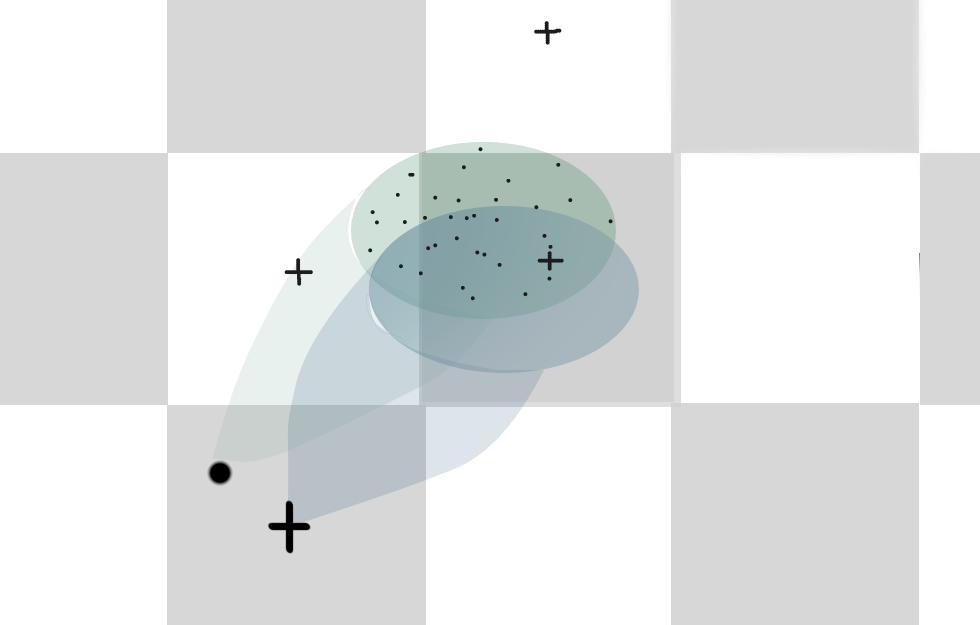
\includegraphics[width = .8\columnwidth]{figs/grid}
	\caption{Depiction of the gridded state space.The mean state of the concrete belief MDP $\bullet$ and the  representative state of the abstract MDP $\boldsymbol{+}$ are given together with an illustration of a stochastic transition. }
\end{figure}

\subsection{Flying in the wind}
\noindent\textbf{Moving point mass.}
    
Consider the linear time invariant system with Gaussian disturbance, given as 
\begin{align}\begin{aligned}
	x^m_{k+1} &= A x^m_{k}+B^mu_{k}+ F^m w_{k}\\
	y^m_{k}&=C^m x^m_{k}+D^m u_{k}+E^m v_{k}\end{aligned}
\end{align}
with matrices $A,B,C,D$ and matrices $F,E$. 
The measurement boise signal $v$ is zero-mean, independently and identically  distributed noise, i.e, $v_k\sim \mathcal{N}(0,I)$.
% \noindent\textbf{Wind disturbance.}
The state transitions are affected by the wind $w_k$. 
We can model the dynamic variations of the wind as filtered noise. 
There are two commonly used models  \citep{richardson2013quantifying},  this includes the von Karman power spectral density,
and the Dryden model.
The former model matches experiment data more than the 
 Dryden model, but the Dryden model can be represented by  a lower order filter.
Consider a filter model to be given as
\begin{align}
	\begin{aligned}
	x_{t+1}^w &= A^w x_{t}^w+ F^w e_{t},\\
	w_{t}&=C^w x_{t}^w+E^w e_{t}.
	\end{aligned}
\end{align}

%\textbf{Full model \& Belief space model.}
The full model is given as follows
%\begin{align} 
%	\begin{bmatrix}
%	x^m_{t+1}	\\x^w_{t+1}
%	\end{bmatrix}
% &= \begin{bmatrix}
% 	A^m 	& F^mC^w\\
% 	0 & A^w
% \end{bmatrix}
%\begin{bmatrix}
%	x^m_{t}	\\x^w_{t}
%	\end{bmatrix}+\begin{bmatrix} B^m \\ 0~ \end{bmatrix} u_{t}+  \begin{bmatrix}
%	F^m E^w \\
%	F^w
%	\end{bmatrix}e_{t}\notag\\
%	y^m_{t}&=\begin{bmatrix} C^m& 0 \end{bmatrix}\begin{bmatrix}
%	x^m_{t}	\\x^w_{t}
%	\end{bmatrix}+D^m u_{t}+E^m v_{t}.
%\end{align}
%This can be written as 
 \begin{align}  \begin{aligned}
x_{t+1}&=A x_{t} + B u_t+ Fe_t\\
y_t&=Cx_t+Du_t+Ev_t\end{aligned} \end{align}
\begin{align}& \mbox{ with }  x_t	= \begin{bmatrix}
	x^m_{t}	\\x^w_{t}
	\end{bmatrix},
A = \begin{bsmallmatrix}
 	A^m 	& F^mC^w\\
 	0 & A^w
 \end{bsmallmatrix}\!, \ 
B = \begin{bsmallmatrix} B^m \\ 0~ \end{bsmallmatrix}\!,\notag \\
&F=\begin{bsmallmatrix}
	F^m E^w \\
	F^w
	\end{bsmallmatrix}\!,\ 
C = \begin{bmatrix} C^m& 0 \end{bmatrix}\!, \ 
D= D^m, \  E = E^m.\notag
\end{align}
 
 \noindent{\textbf{}}

    
    \red{[STEPS to do]
  \begin{enumerate}
  	\item Use upper\&lower bound on covariance to define standard LTI gaussian fully observable system (if exists ) 
  	\item The covariance of the innovation sequence is given in Anderson, Optimal filtering 4.13.
  	\item For observable LTI system design controller
  	\item translate scLTL to DFA
  	\item compute cross product
  	\item Value iteration
  	\item implementation
  \end{enumerate}
  
  
  }
    
  
\section{Conclusions}


%% Bibiliography %%%%%%%%%%%%%%%%%%%%%%%%
\bibliography{AliAgha,references}

%%%%%%%%%%%%%%%%%%%%%%%%%%%%%%%%%%


\appendix

\section{Kalman filtering}
Consider a Gaussian LTI system:
 \begin{align}  \begin{aligned}
x_{k+1}&=A x_{k} + B u_t+ w_k,\\
z_k&=Cx_k+Du_k+v_k.\end{aligned} \end{align}
with $w_k\sim \mathcal N(0, \mathcal W)$ and $v_k\sim \mathcal N (0,\mathcal V)$.

At $k=0$, we know $x_0\sim \init$ with $\init:=\mathcal N(x_\init,P_\init)$.
Thus,  before receiving a measurement $z_0$, the distribution of the belief is defined as $\CA N(x_{0|-}, P_{0|-})$
\begin{align}
	\hat x_{0|-}&:= x_\init\\
	P_{0|-}&:= P_{\init}
\end{align}
After receiving the measurement $z_0$, this is updated to $\CA N(\hat x_{0|0}, P_{0|0})$
\begin{align}
	\hat x_{0|0}&:= x_\init+ L_0 (z_0-Cx_\init)\\
	P_{0|0}&:=(I-L_0 C) P_{\init}(I-L_0 C)^T+L_0\CA V L_0^T\\
	& \mbox{ with } L_0=P_{\init}C^T\left(CP_{\init}C^T+\mathcal V\right)^{-1}
\end{align}
We represent the belief state  $\CA N(\hat x_{0|0}, P_{0|0})$ by $b_0:=(\hat x_{0|0}, P_{0|0})\in\mathbb R^n\times \mathbb S^n$.

The dynamics of the Kalman filter are given as
	\begin{align*}
	&&\textbf{Predict} \qquad \hat x_{k|k-1}&=A\hat x_{k-1|k-1}+Bu_{k-1}\\
	&&P_{k|k-1}&=AP_{k-1|k-1}A^T+\mathcal W
\\
	&&\textbf{Update} \  \qquad e_{k}&=z_k-C \hat x_{k|k-1}\\
	&&S_k&=CP_{k|k-1}C^T+\mathcal V\\
	&&L_{k}&=P_{k|k-1}C^TS_k^{-1}\\
	&&\hat x_{k|k}&=\hat x_{k|k-1}+L_ke_k\\
	&&P_{k|k}&=(I-L_kC)P_{k|k-1}\\
	\end{align*}
	\mbox{Joseph Formula  }
	\begin{align*}
	&&P_{k|k}&=(I-L_kC)P_{k|k-1}(I-L_kC_k)^T+L_k\mathcal V_kL_k^T\\
		\end{align*}
\mbox{Observability based }
	\begin{align*}
	&& P_{k|k}^{-1}&=P_{k|k-1}^{-1}+C_k^T \mathcal  V_k^{-1}C_k
	\end{align*}

Though the covariance of the belief state is defined as 
	\begin{align*}
	&&P_{k|k}&=(I-L_kC)P_{k|k-1}(I-L_kC_k)^T+L_k\mathcal V_kL_k^T, \\
		\end{align*}
		The update equations for $P_{k|k-1}$ are more well know:
			\begin{align*}
	&&P_{k+1|k}&=(A-K_kC)P_{k|k-1}(A-K_kC_k)^T+K_k\mathcal V_kK_k^T 
		\end{align*}
		with $K_k=AL_k$.
		
Hence, the belief state is updated as
\begin{align}
	&&\hat x_{k|k}&=A\hat x_{k-1|k-1}+Bu_{k-1}+L_ke_k\\
	&&P_{k|k}&=f(P_{k-1|k-1})
\end{align}
We now want to model the random variable $s_k=L_ke_k$. We know that $s_k$ evolves as a zero mean Gaussian distributed stochastic process.
Further 
\begin{align*}
	\Ex [s_k]=0\\
	\Ex [s_ks_k^T]=L_k	\Ex [e_ke_k^T]L_k^T, \mbox{ and } \Ex [e_ke_k^T]=S_k \\
	e_k = C\left(x_k- \hat x_{k|k-1}\right)+v_k\\
	\Ex [e_ke_k^T] = C P_{k|k-1} C^T + \CA V\\
		\Ex [s_ks_k^T]=L_k S_k L_k^T,\\
				\Ex [s_ks_k^T]= P_{k|k-1} C^T S_k^{-1} C P_{k|k-1},\\
								\Ex [s_ks_k^T]= P_{k|k-1} C^T \left(CP_{k|k-1}C^T+\mathcal V\right)^{-1} C P_{k|k-1},\notag\\
\Ex [s_ks_k^T]= P_{k|k-1}-P_{k|k}\notag
\end{align*}


\begin{align}
	&\text{concrete:}\left\{\begin{aligned}
		&&\hat x_{k|k}&=A\hat x_{k-1|k-1}+Bu_{k-1}+ P_{k|k-1} C^T  \bar{s}_k\notag \\
		&&&\mbox{with } \bar{s}_k\sim \CA N (0,S_k^{-1}) \notag 
	\end{aligned}\right.	\\
&		\text{abstract 1:}\left\{\begin{aligned}
		&&\hat x_k &=A\hat x_{k-1} +B\hat u_{k-1} + \bar P  C^T  \hat{s}_k\notag \\
		&&&\mbox{with } \hat{s}_k\sim \CA N (0,\hat{S}_{inv}) \notag 
	\end{aligned}\right.	
\end{align}
Define  $\Delta_k:=P_{k|k-1} -\bar P $,  then  $S_k=\left(C\bar PC^T+C\Delta_kC^T+\mathcal V\right)$.
Find maximal $\hat{S}_{inv}$ such that $\hat{S}_{inv}\preceq S_k^{-1}$



\end{document}

